\subsection{Pharmacokinetics}

In this section, I describe pharmacokinetic as it will be used in the proposed research.  I will explain aspects of both pharmacokinetic and pharmacodynamic models, and how the two are related.  One and two compartment model(s) for pharmacokinetics will be constructed and interpreted.


\subsubsection{Pharmacokinetics v. Pharmacodynamics}

The phases between drug administration and emergence of the desired effect can be broadly placed into one of two areas of study.  The area of study which is concerned with relationship between dose administration and achievement of particular concentrations in the body is known as \textit{pharmacokinetics}, while the area of study concerned with the arrival of the drug at it's site of action, the onset of the desired effect, as well as the magnitude and duration of that effect is known as  \textit{pharmacodynamics} \cite{rosenbaum2016basic}.  

\subsubsection{A One Compartment Pharmacokinetic Model}

To analyze the time course of drug concentrations in various parts of the body, compartmental models are often used.  These models posit that the body (or relevant organs/systems of the body) is comprised of compartments from which drug can flow in and out. The rates at which the drug can enter and exit each compartment are specified, and a differential equation for each compartment can be written down and solved using methods outlined in \cref{sec:ODE}.

The simplest example of these models is the one compartment pharmacokinetic model.  The model posits the following \cite{wakefield1992bayesian}:  
%
\begin{itemize}
\item The rate of drug absorption from the gut ($ G  $) into the blood plasma ($ C $) is proportional to the amount of drug in the gut and that is the proportionality constant is $ k_a $, in units $ \text{hours}^{-1} $.  

\item The rate of elimination from the blood plasma is proportional to the amount of drug in the plasma compartment with proportionality constant $ k $, in units $ \text{hours}^{-1} $.

\item The volume of plasma in the body is $ V $, in units litres.

\item The bioavailability of the drug (i.e. the fraction of drug absorbed into the blood serum) is 1.
\end{itemize}
%
 A visual representation of this model is shown in \cref{compartmental_model}.

\begin{figure}[h!]
	\centering
	
	\tikzstyle{int}=[draw, fill=white, minimum size=2em]
	\tikzstyle{init} = [pin edge={to-,thin,black}]
	
	
	\begin{tikzpicture}[node distance=2.5cm,auto,>=latex']
	
	
	\node [int] (a) {$G$};
	\node (b) [left of=a,node distance=2cm, coordinate] {a};
	\node [int] (c) [right of=a] {$C$};
	\node [coordinate] (end) [right of=c, node distance=2cm]{};
	\path[->] (a) edge node {$k_a$} (c);
	\draw[->] (c) edge node {$k$} (end) ;
	\end{tikzpicture}
	\caption[Pharmacokinetic compartmental diagram]{A compartmental diagram for a one compartment pharmacokinetic model.  Arrows indicate the direction of flux.  Flux is proportional to the concentration in each compartment, with proportionality constant indicated over the arrows.}
	\label{compartmental_model}
\end{figure}

The pharmacokinetic model described in \cref{compartmental_model} can be written as a system of differential equations, namely
%
\begin{alignat*}{3}
	\dfrac{dG}{dt} &= -k_aG \>, \quad  &&G(0) = \dfrac{D}{V} \\
	\dfrac{dC}{dt} &= k_aG - kC \>,   \quad  &&C(0) = 0
\end{alignat*}
%
 It can be shown that the solution for the concentration of drug in the blood at a given time is 

\begin{equation}\label{onecompartment_PKPD}
	C(t) = \dfrac{D}{V}\dfrac{k_a}{k - k_a}\Big(e^{-k_at} - e^{-kt}\Big) \>.
\end{equation}

\begin{figure}[h!]
	\centering
	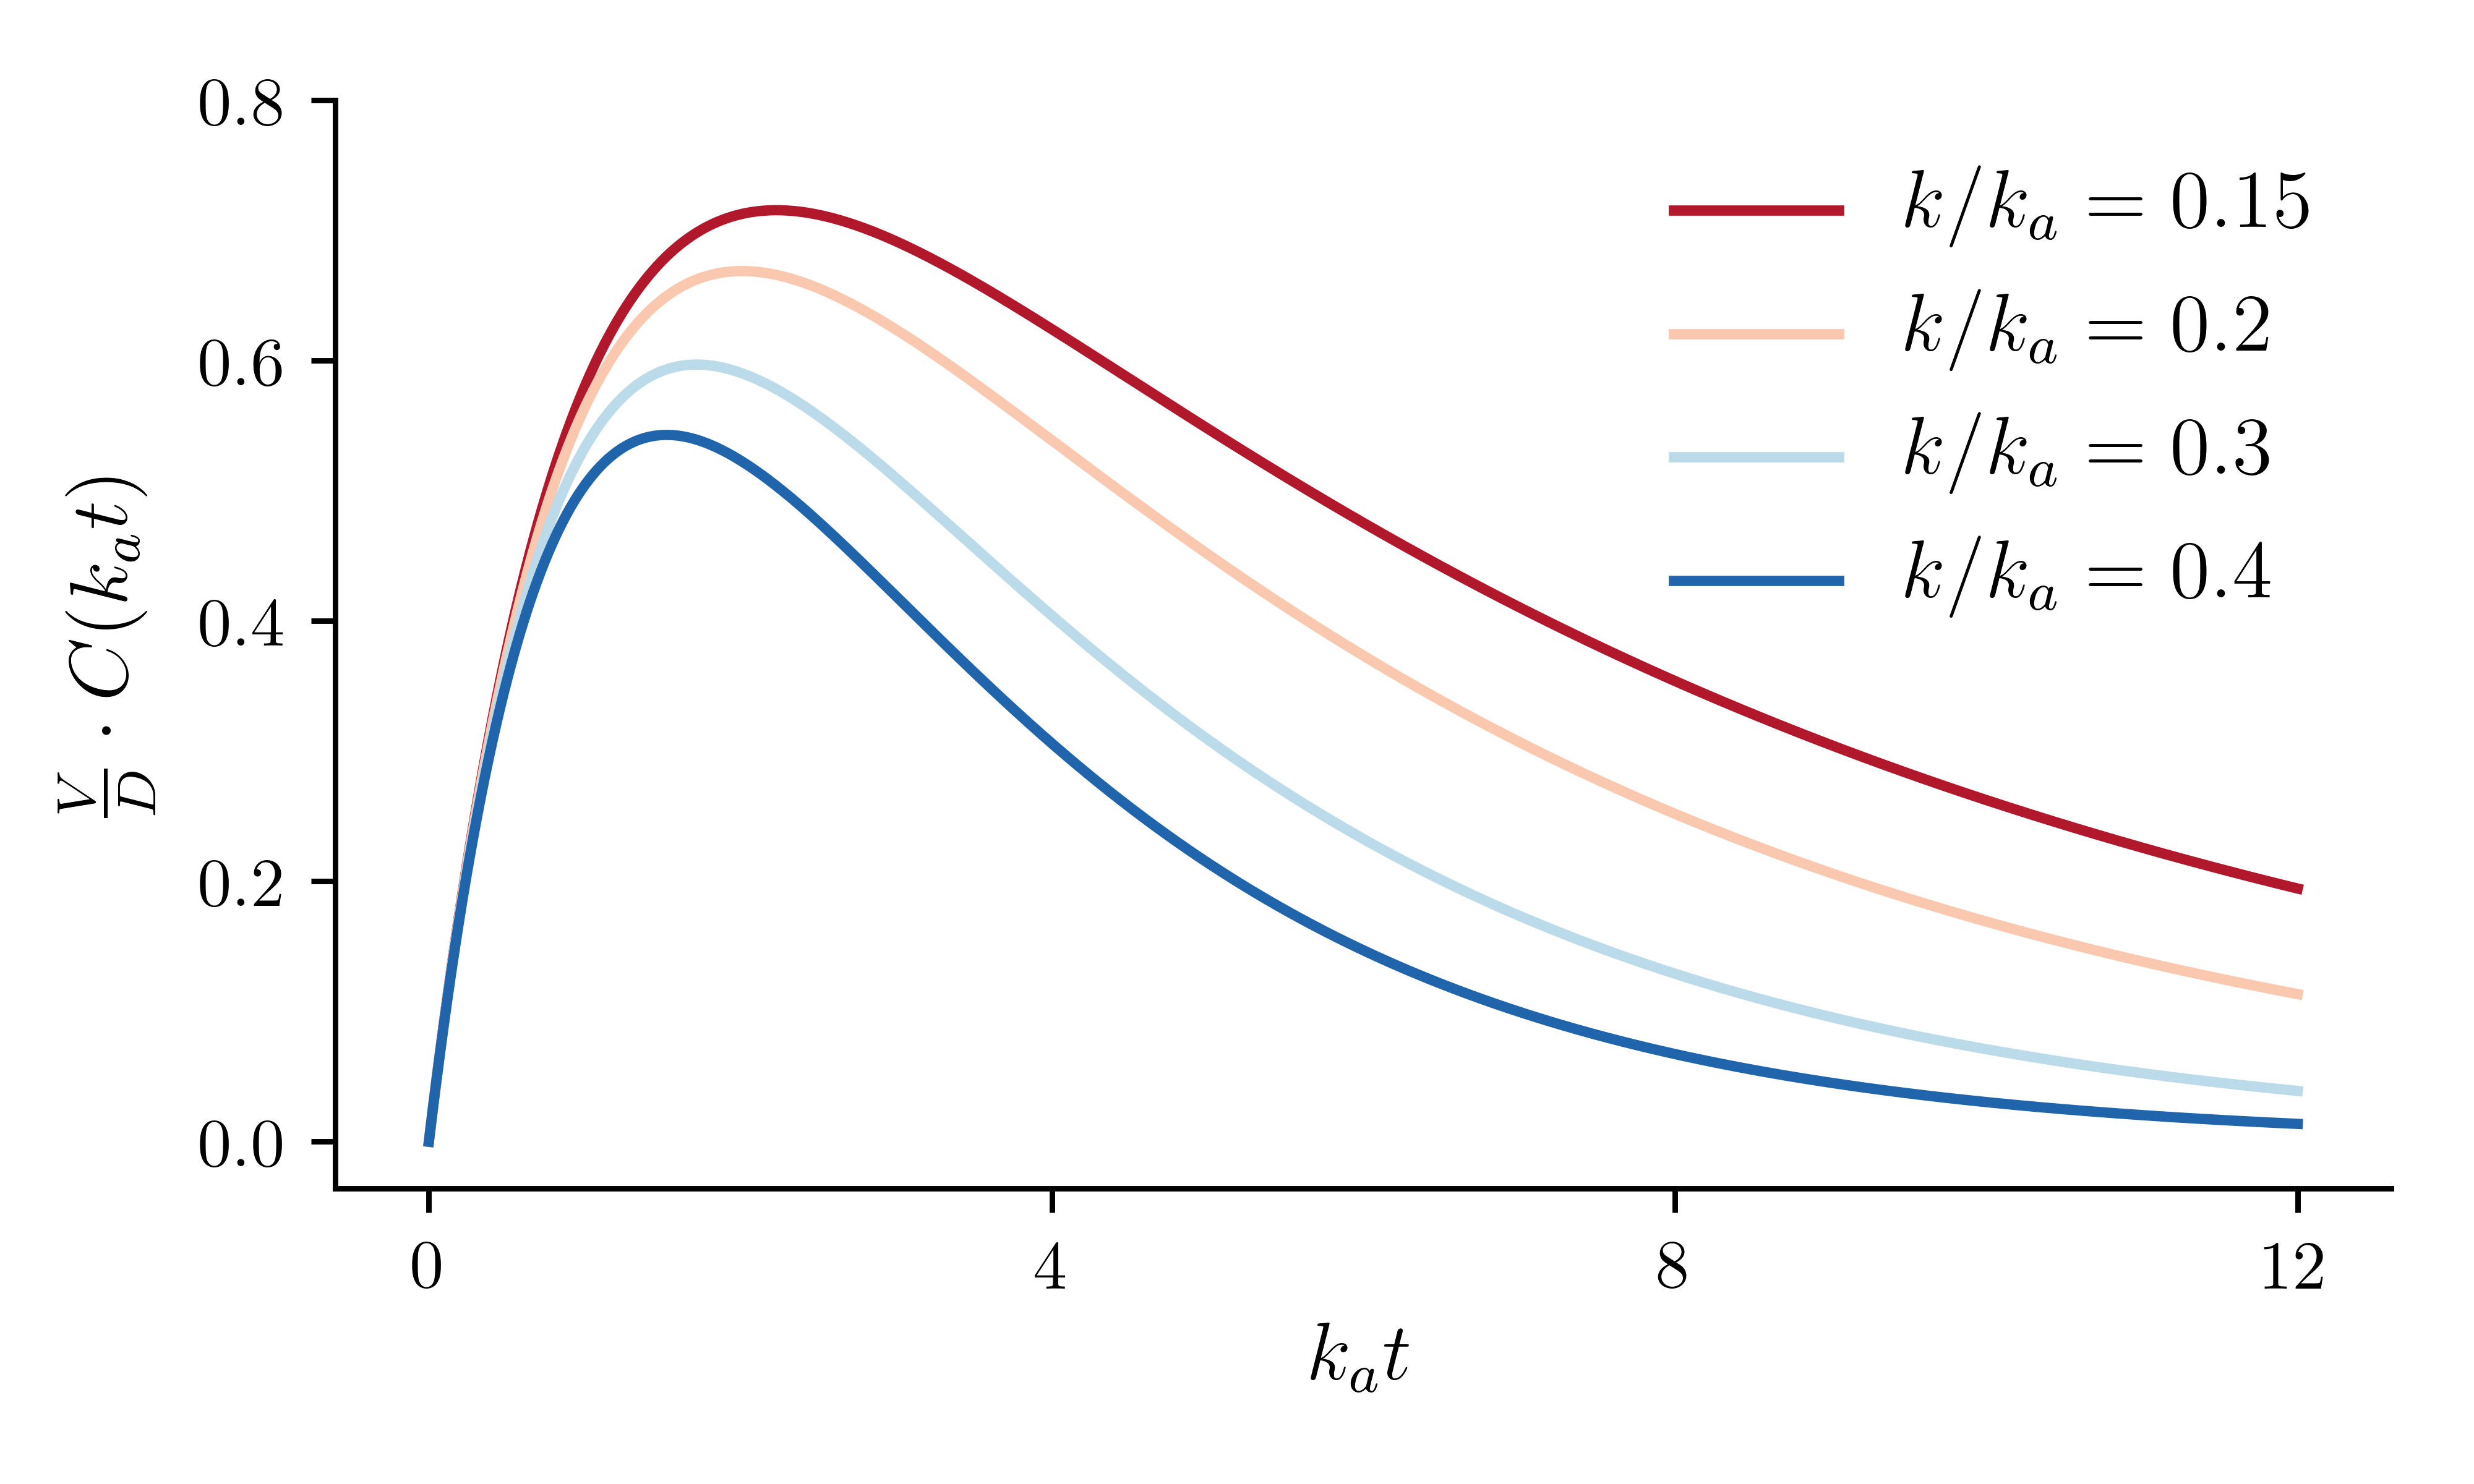
\includegraphics{Figures/pkcureves.png}
	\caption[Non-dimensionalized solutions to pharmacokinetic differential equation]{\Cref{onecompartment_PKPD} under various parameterizations.  Here, $ C(t) $ has been scaled by a factor of $ V/D $ and time has been scaled by a factor of $ k_a $.  This is called a \textit{non-dimensionalization} of the system.  Applied mathematicians non-dimensionalize dynamical systems in order to normalize and compare common properties of different implementations of the same system.  It is clear from this plot that as $ k/k_a \rightarrow 1^- $, the maximum amount of drug in the blood serum compartment will be smaller and will occur sooner after administration.  This is a common property of all systems with constant $D/V$. }
	\label{fig:pkcureves}
\end{figure}


\subsubsection{A Two Compartment Pharmacokinetic Model}

The model presented above can be extended to include a second compartment, $C_2$ which may be the concentration of the drug at it's site of action.  The assumptions for the previous models still hold, but now the model allows for flux of drug between the blood serum compartment and site of action compartment, as well as elimination of the drug from both compartments. Shown in \cref{two_compartmental_model} is a compartmental diagram for the two compartment pharmacokinetic model.

\begin{figure}[h!]
	\centering
	
	\tikzstyle{int}=[draw, fill=white, minimum size=2em]
	\tikzstyle{init} = [pin edge={to-,thin,black}]
	
	
	\begin{tikzpicture}[node distance=2.5cm,auto,>=latex']
	
	\node [int] (G){$G$};
	\node [int] (C1)[right of = G]{$C_1$};
	\node [int] (C2)[right of = C1]{$C_2$};
	\node [coordinate] (C2_exit) [below of=C2, node distance=2cm]{};
	\node [coordinate] (C1_exit) [below of=C1, node distance=2cm]{};
	 
	 \path[->](G) edge node {$k_a$} (C1);
	 \path[->, bend left](C1) edge node {$k_{12}$} (C2);
	 \path[<-, bend right](C1) edge node {$k_{21}$} (C2);
	 \path[->](C1) edge node {$k_1$} (C1_exit);
	 \path[->](C2) edge node {$k_2$} (C2_exit);
	\end{tikzpicture}
	\caption{Two compartment pharmacokinetic model.}
	\label{two_compartmental_model}
\end{figure}

The differential equations governing this system are

\begin{alignat*}{3}
\dfrac{dG}{dt} &= -k_aG \>, \quad  &&G(0) = \dfrac{D}{V} \\
\dfrac{dC_1}{dt} &= k_aG + k_{21}C_2 - (k_1  + k_{12})C_1 \>,   \quad  &&C_1(0) = 0\\
\dfrac{dC_2}{dt} &= k_{12}C_1 - (k_{21} + k_2)C_2\>,   \quad  &&C_2(0) = 0
\end{alignat*}

These models are easily constructed to arbitrarily many compartments, but with more compartments comes a need for more data, which may not always be feasible.

